\documentclass[main.tex]{subfiles}
\begin{document}

\section{ Частотные критерии устойчивости Михайлова и Найквиста }
5 марта 2021 г. \\

Темы важные, непростые.
Возможно, даже центральные! \\

Устойчивость -- основное свойство системы.
Как правило, все системы должны быть устойчивы.
Истребитель, в отличие от гражданского самолёта, в свободном полёте неустойчив, НО с помощью обратной связи мы вновь делаем его устойчивым!

\textbf{Напоминание:} для устойчивости линейной динамической системы достаточно выполнения условия
$$ \boxed{Re \lambda_i < 0} $$
где $ \lambda_i : \alpha(\lambda_i) = 0 $

Проверять корни характеристического полинома -- занятие неблагодарное.
Есть необходимое условие Стодола, а также н. и д. условие Гурвица.
Их дополняет критерий Льенара-Шипара.

\subsubsection{Частотные критерии. Введение}

На прошлом занятии мы разобрали, что такое частотные характеристики.
Зачем они нужны, если есть алгебраические?
Когда порядок системы большой (10, 100, ...), задача вычисления большого числа определителей также неблагодарная.
А на базе некоторых характеристик, которые мы будем называть \emph{годографами}, можно определить устойчивость проще.
Причём будет достаточно найти годографы лишь приближённо.
Знак определителя не найти с помощью приближённых вычислений!

\subsection{Критерий Михайлова}
1938 год.

Частотные характериристики основаны на \textbf{принципе аргумента} из теории функции комплексной переменной: приращение аргумента функции при обходе области
$$ \Delta \arg f(z) = 2 \pi (N - P) $$
здесь $N$ -- число нулей и $ P $ -- число полюсов внутри области.

Докажем в одном частном случае -- когда функция $f(z)$ -- полином, а $p$ пробегает по мнимой оси (нам этого достаточно).

$$ \alpha(p) = a_0 p^n + ... + a_n \overset{\text{th.  Безу}}= a_0 \prod_i (p - p_i), \thickspace \alpha(p_i) = 0 $$
где $ \alpha(p) $ -- характеристический полином, знаменатель некоторой передаточной функции $ H(p) = \frac{\beta(p)}{\alpha(p)} $.

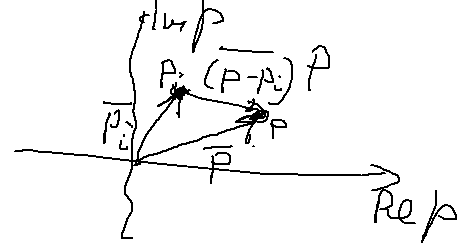
\includegraphics[width=.4\linewidth]{lec6/01_polynome_roots}

Пусть $p = j \omega $ (хотим располагаться на мнимой оси).
Пусть также для определённости $ a_0 > 0 $, т. е. $ \arg a_0 = 0 $.

Аргумент произведения есть сумма аргументов.
Аргумент $ a_0 $ равен нулю, если это положительное вещественное число.
$$ \arg \alpha(j \omega) = \sum_{i=1}^{n} \arg (j \omega - p_i) $$
Найдём приращение аргумента при перемещении точки от $ - \infty $ до $ + \infty $ по комплексной оси
$$ \Delta \arg \alpha(j \omega) |_{-\infty}^\infty = \sum_i \Delta \arg (j \omega - p_i) |_{-\infty}^\infty $$

Изобразим корни уравнения на комплексной плоскости:

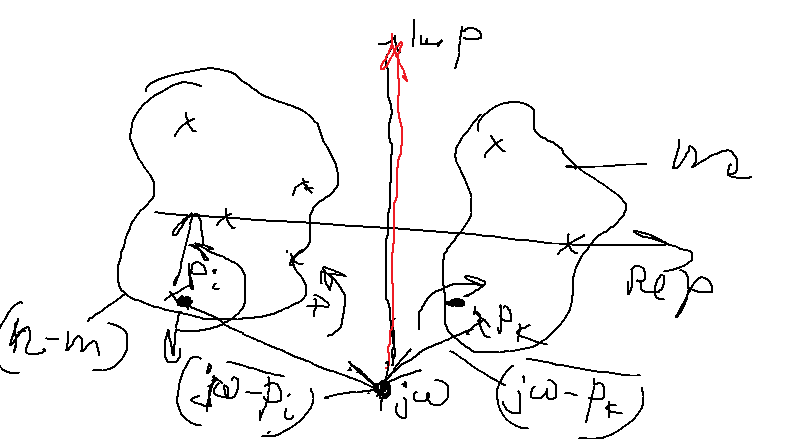
\includegraphics[width=.6\linewidth]{lec6/02_roots_jw}

Хотим посмотреть на приращение аргумента от каждого слагаемого $ p - p_i $ (и затем эти приращения просуммировать).
Пусть в правой полуплоскости $ m $ корней $ \Rightarrow $ в левой $ n - m $ (общий порядок $n$).

Условимся считать за положительное направление поворот против часовой стрелки.
От каждого вектора из левой полуплоскости приращение угла поворота при проходе $ \omega $ от $ - \infty $ до $ + \infty $ есть $ \pi $, от каждого правого -- $ \pi $. Тогда

$$ \Delta \arg \alpha(j \omega) |_{-\infty}^\infty = \pi (n - m) - \pi \cdot m = \pi (n - 2 m)  $$
Принцип аргумента в нашем частном случае доказан. \\

Нарисуем один из возможных годографов, то есть кривую $ \alpha(j \omega) |_{-\infty}^\infty $ в осях $ Re(\alpha(j \omega)), Im(\alpha(j \omega)) $.

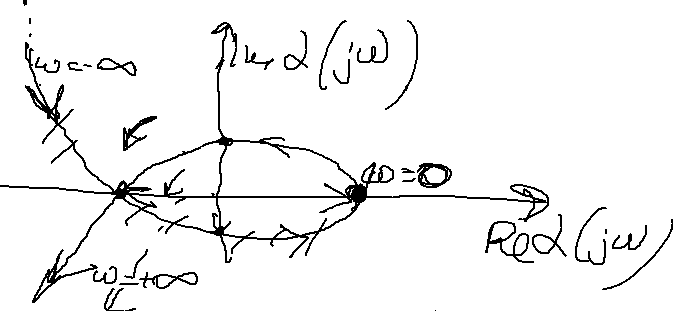
\includegraphics[width=.5\linewidth]{lec6/03_mikhailov_godograph}

Геометрическое место точек, образованное значениями полинома $ \alpha(j \omega) $ (точнее, её половину), называют \emph{кривой Михайлова}.

Пример.

\begin{align*}
    & \alpha(p) = p^2 + p + 1 \\
    & \alpha(j \omega) = 1 - \omega^2 + j \omega \\
    & \text{обозначим } X(\omega) = 1 - \omega^2, \thickspace Y(\omega) = \omega \\
    & \alpha(j \omega) = X(\omega) + j Y(\omega) \\
    & X(\omega) = X(-\omega) \Rightarrow \text{ годограф симметричен относительно вещественной оси} \\
    & Y(\omega) = Y(- \omega) \Rightarrow Y(\omega = 0) = 0 \\
\end{align*}

Приращение аргумента при движении по годографу от $ \omega = - \infty $до $ \omega = \infty $ есть$ 3 \pi $.
Поскольку кривая симметрична, можно рассматривать только его половину $ \alpha(j \omega) |_0^\infty $

На <<половинной>> кривой для нашего примера приращение аргумента $ 3\frac{\pi}{2} $, а в общем случае

\begin{equation}\label{eq:mikhailov}
	\boxed{ \Delta \arg \alpha (j \omega) |_0^\infty = \frac{\pi}{2} (n - 2m) }
\end{equation}

Для устойчивости необходимо и достаточно, чтобы $ m = 0 $ (нет правых, неустойчивых корней):
\begin{equation}\label{eq:mikh1}
\boxed{ \Delta \arg \alpha(j \omega) |_0^\infty = \frac{\pi}{2} n }
\end{equation}
Для асимптотической устойчивости также нужно, чтобы не было корней на мнимой оси:
\begin{equation}\label{eq:mikh2}
	\boxed{ \alpha(j \omega) \ne 0 }
\end{equation}
(т. о. годограф не должен проходить через начало координат). Пример хорошего годографа:

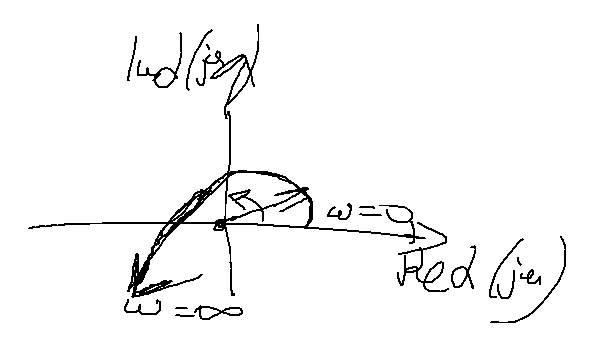
\includegraphics[width=.5\linewidth]{lec6/04_mikhailov_polyn_godograph}

Формулы \eqref{eq:mikh1} и \eqref{eq:mikh2} вместе и есть критерий Михайлова.

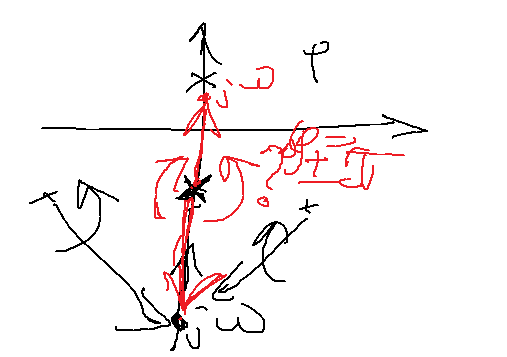
\includegraphics[width=.5\linewidth]{lec6/05_mikhailov_imaginary_roots}

Пояснение к формуле \eqref{eq:mikh2}:
если корень на мнимой оси, то приращение аргумента при его обходе -- $\pi$, но мы не знаем, с каким знаком.
То есть неопределённость: $ \Delta \arg j \omega = ? $

Это как деление на ноль -- если определим как предел, будет непонятно, какой знак: $ \frac{1}{0} = \lim\limits_{\varepsilon \to 0} \frac{1}{\varepsilon} = \pm \infty \Rightarrow $ неопределённость, не можем так определить. \\

\textbf{Замечания:}

\begin{enumerate}[noitemsep]
	\item Для устойчивой системы кривая Михайлова имеет вид спирали, которая стартует на вещественной оси, всё время монотонно раскручивается в одном направлении и заканчивается в квадранте $ n $ (т. е. $ \Delta \phi = n\frac{\pi}{2} $), $n$ -- порядок полинома $\alpha$.

    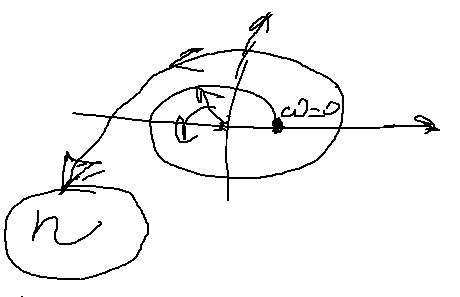
\includegraphics[width=.4\linewidth]{lec6/07_mikh_revolutions}

    Пример:

    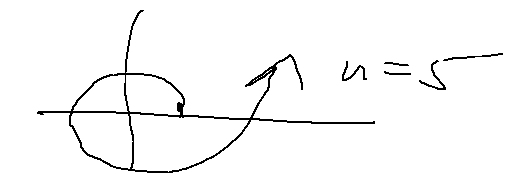
\includegraphics[width=.4\linewidth]{lec6/09_mikh_example1}

    Следующий годограф невозможен, если система устойчива:

    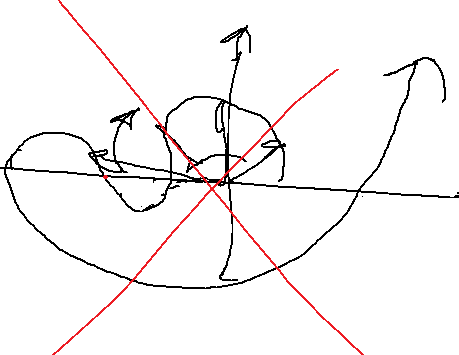
\includegraphics[width=.4\linewidth]{lec6/08_mikh_wrong_revolutions}

	Почему спираль монотонно раскручивается?
	Изменение аргумента от всякого корня с $ Re < 0 $ есть монотонная функция, и сумма их тоже.

    Смотрите, как замечательно:
    нам неважно, по каким точкам проходит кривая, важен только вид и с точностью до квадранта -- точка, в которой она заканчивается.
	\item В любом случае, вне зависимости от устойчивости, угол поворота кратен $ \pi $ (в силу формулы \eqref{eq:mikhailov})
	\item Если система неустойчива, то критерий Михайлова -- единственный, который позволяет найти число неустойчивых корней $ m $.
    Это зачастую важно: к примеру, система десятого порядка и только один корень неустойчивый $ \Rightarrow $ наверняка можно ввести какое-то дополнительное звено и привести её в устойчивое состояние.
    Если же неустойчивых десять, то это хуже.
	$m$ можно найти из \eqref{eq:mikhailov}
\end{enumerate}

\textbf{Пример.}

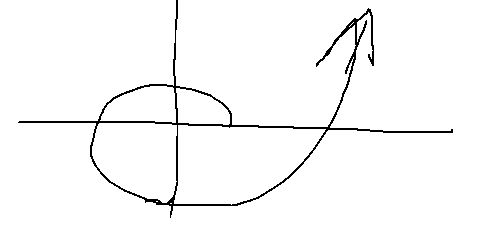
\includegraphics[width=.4\linewidth]{lec6/10_mikh_example4a}

При $ n = 7 $ система на картинке неустойчива ( $ \Delta \phi = \frac{5}{2} \pi \overset{\eqref{eq:mikhailov}}\Rightarrow m = 1 $, один неустойчивый корень).

\textbf{Иной пример.}

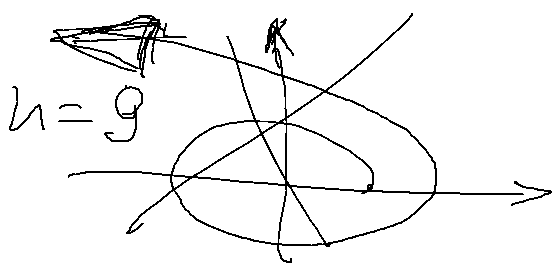
\includegraphics[width=.4\linewidth]{lec6/11_mikh_example4b}

При $ n = 9 $ такой годограф невозможен.
Такой системы просто не может быть, ни устойчивой, ни неустойчивой.

\textbf{Вывод:} приращение аргумента зависит от чётности порядка системы.
Если порядок системы нечётный, годограф должен заканчиваться в нечётном квадранте (вне зависимости от того, устойчива ли система). \\

\textbf{Более конструктивный пример:} инерционное звено

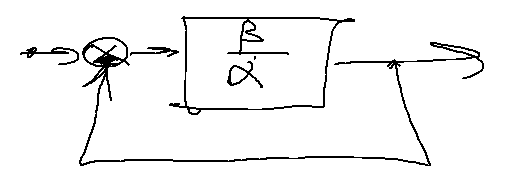
\includegraphics[width=.4\linewidth]{lec6/16_mikh_bound_scheme}

\begin{align*}
	&  H(p) = \frac{1}{Tp + 1} \\
	& \alpha(p) = Tp + 1 \\
	& \alpha(j \omega) = 1 + j \omega T \\
\end{align*}

Кривая здесь -- просто прямая:

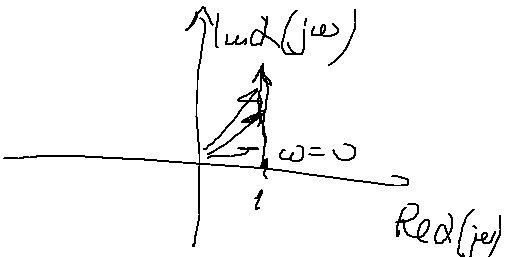
\includegraphics[width=.4\linewidth]{lec6/12_mikh_example5a}

$$ \begin{cases}
    \Delta \phi = \frac{\pi}{2} \\
    n = 1
\end{cases} \overset{\eqref{eq:mikhailov}}\Rightarrow m = 0, \text{система устойчива} $$

Если же  $ H(p) = \frac{1}{Tp - 1} $, рисунок зеркальный относительно вещественной оси.

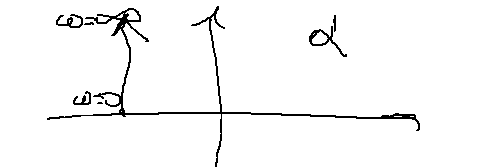
\includegraphics[width=.4\linewidth]{lec6/13_mikh_example5b}

Система при этом становится неустойчивой ($ \Delta \phi = -\frac{\pi}{2} $, один неустойчивый корень).

\subsubsection{Критерий Михайлова. Граница устойчивости}

Граница устойчивости -- ситуация, когда среди корней $ \alpha $ нет положительных, но некоторые находятся на мнимой оси.

Как с помощью критерия Михайлова идентифицировать систему, находящуюся на границе устойчивости?
Необходимое, но не достаточное условие: годограф проходит через ноль.

\textbf{Пример:} $ n=4 $.

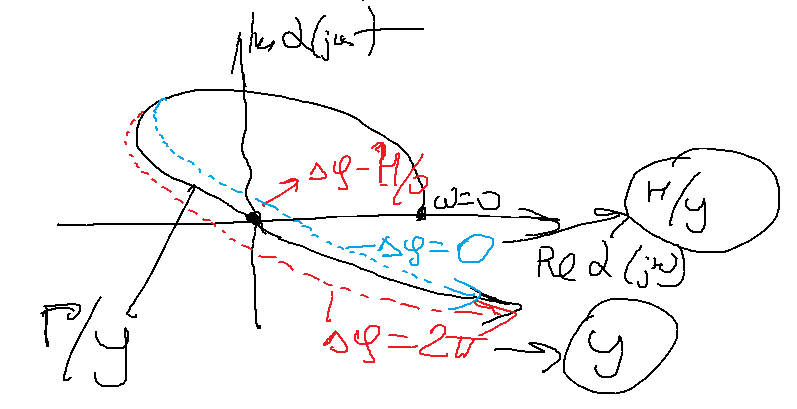
\includegraphics[width=.4\linewidth]{lec6/15_mikh_bound_godograph}

Пошевелим немного годограф в одну сторону (красная кривая) $ \Rightarrow $ система становится устойчивой ($ \Delta \phi = 2 \pi $).
Пошевелим в другую $ \Rightarrow  \Delta \phi = 0$, система неустойчива.

Смотрите-ка, мы на границе устойчивости!

Если бы порядок был $ n = 6 $ (а не $4$), то при смещении в одном случае (синяя кривая) было бы 3 неустойчивых корня с $Re \lambda > 0$; при смещении в другую сторону (красная кривая) был бы 1 неустойчивый корень:

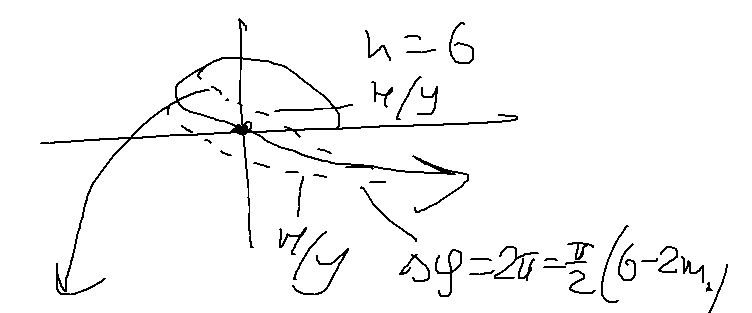
\includegraphics[width=.4\linewidth]{lec6/15_mikh_bound_godograph2}

Следовательно, при $ n = 6 $ система не находится на границе устойчивости.

Зная годограф и $n$, можно восстановить картину расположения корней:
если годограф подвинуть вниз, то $ \Delta \phi = 2 \pi \overset{\eqref{eq:mikhailov}}\Rightarrow m_1 = 1  $; если вверх, то $ \Delta \phi = 0 \overset{\eqref{eq:mikhailov}}\Rightarrow m_2 = 3  $.

Т. о. два корня находятся на мнимой оси и при движении смещаются вправо / влево, один корень справа от мнимой оси (неустойчивый, отмечен красным) и три слева (возможно, комплексные).

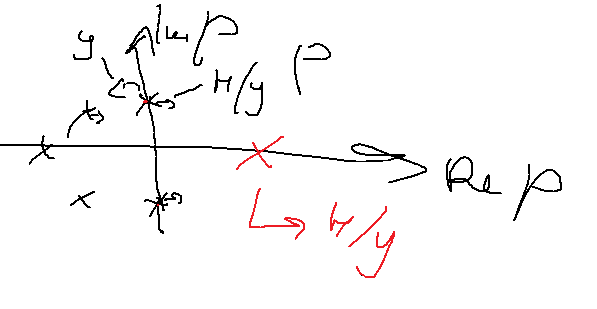
\includegraphics[width=.4\linewidth]{lec6/14_mikh_bound}

\subsubsection{Примеры. Критерий Михайлова для передаточной функции замкнутой цепи}

\textbf{Пример 1.} Пусть
$$ H_{\text{разомкн}} = \frac{K}{p(Tp + 1)} $$
и система с отрицательной единичной обратной связью:

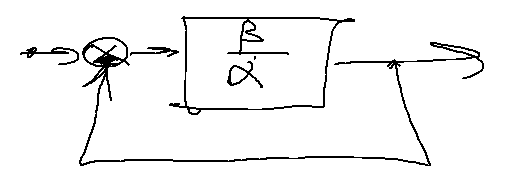
\includegraphics[width=.4\linewidth]{lec6/16_mikh_bound_scheme}

Тогда
$$ H_{\text{замкн}} = \frac{\frac{\beta}{\alpha}}{1 + \frac{\beta}{\alpha}} = \frac{\beta}{\alpha + \beta} = \frac{\beta}{\alpha_{\text{з}}} $$
Отсюда (в общем случае, вне зависимости от вида $ H_{\text{разомкн}} $):
$$ \boxed{ \alpha_{\text{з}} = \alpha + \beta } $$

Проверяем устойчивость по критерию Михайлова:
\begin{enumerate}[noitemsep]
    \item $ \alpha_{\text{з}}(p) = Tp^2 + p + K $
    \item $ \alpha_{\text{з}}(j \omega) = K - T \omega^2 + j \omega $
\end{enumerate}

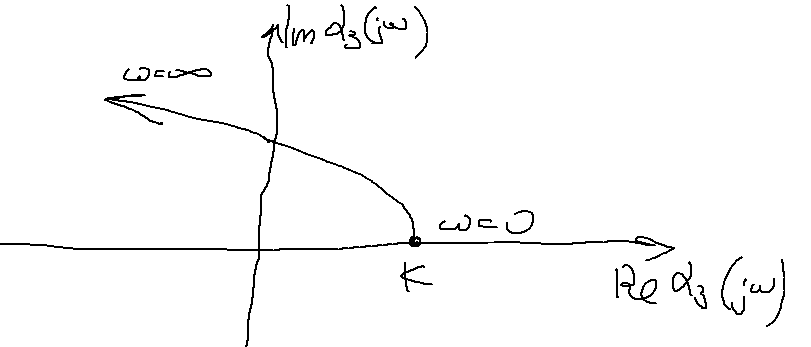
\includegraphics[width=.4\linewidth]{lec6/17_mikh_bound_godograph3}

$$ \Delta \phi = \pi \Rightarrow \text{ система устойчива } $$

\textbf{Пример 2.} Требуется найти $ K_{\text{крит}} $ (критическое значение константы, при котором система на границе устойчивости) для системы третьего порядка:
$$ H_{\text{разомкн}} = \frac{K}{p(T_1 p + 1)(T_2 p + 1)} $$

где константы $ T_1, T_2 > 0 $.

Решение:

\begin{align*}
	& \alpha = T_1 T_2 p^3 + (T_1 + T_2) p^2 + p + K \text{ (необх. условие Стодола выполнено)} \\
    & \alpha(j \omega) = K - (T_1 + T_2) \omega^2 + j \omega (1 - T_1 T_2 \omega^2) \\
\end{align*}

Рисуем годограф: стартуем из точки на вещественной оси; в пределе при $ \omega \to \infty $ находимся в третьем квадранте, причём вещественная часть будет больше мнимой.

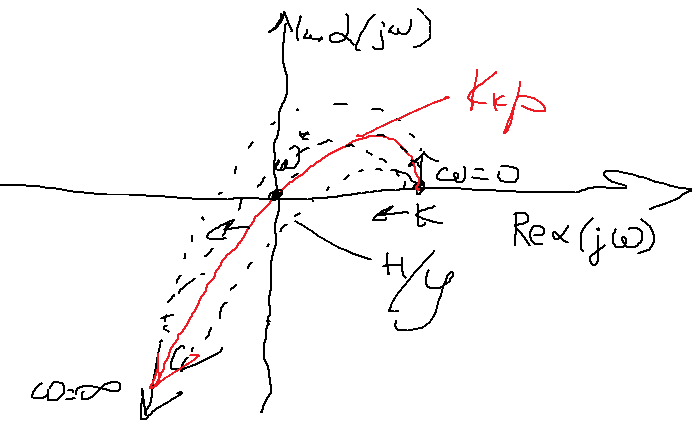
\includegraphics[width=.4\linewidth]{lec6/18_mikh_bound_godograph4}

Ищем критическое значение константы.

\begin{align*}
    & K_{\text{крит}} : \exists \omega^* : \alpha(j \omega^*) = 0 \\
    & j \omega^* (1 - T_1 T_2 \omega^{*2}) = 0 \Rightarrow \omega^* = \frac{1}{\sqrt{T_1 T_2}} \\
    & K - (T_1 + T_2) \omega^{*2} = 0 \Rightarrow K_{\text{крит}} = \frac{T_1 + T_2}{T_1 T_2} \\
\end{align*}

Система устойчива, если $ K < K_{\text{крит}} $.

Естественно, такой же вывод можно сделать по критерию Гурвица -- произведение средних коэффициентов должно быть в устойчивой системе больше произведения крайних:
$$ T_1 + T_2 > T_1 T_2 $$

\subsection{Критерий Найквиста}
Найквист (Nyquist, 1932, чуть пораньше Михайлова) -- американец.
Чуть попроще критерия Михайлова + преимущество: можем определить число неустойчивых корней.

\textbf{Сравнение:} Михайлов работает со знаменателем замкнутой передаточной функции $ \alpha_{\text{з}}(j \omega) $, Найквист -- с разомкнутой $ H_{\text{разомкн}} = \frac{\beta(j \omega)}{\alpha(j \omega)} $.
Строить годограф полинома, конечно, проще, чем дроби, в этом недостаток Найквиста; но зато, как правило, передаточная функция разомкнутой цепи есть произведение элементарных передаточных функций (т. к. последовательное соединение): $ H_{\text{разомкн}} = \prod H_i $.
По трудоёмкости в среднем примерно одно и то же. \\

Построим вспомогательную функцию
$$ \Psi(p) = 1 + H_{\text{разомкн}(p)} $$
Здесь $ H_{\text{раз}}=\frac{\alpha}{\beta} $:

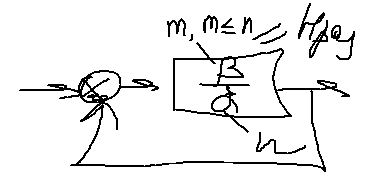
\includegraphics[width=.4\linewidth]{lec6/19_nyquist_example1}

$$ \Psi(p) = 1 + H_{\text{разомкн}} = 1 + \frac{\beta}{\alpha} = \frac{\alpha + \beta}{\alpha} = \frac{\alpha_{\text{з}}}{\alpha} $$
Порядок знаменателя $n$, числителя -- $ m \le n \Rightarrow $ порядок $ \alpha_{\text{з}} $ тоже $ n $.

Хотим найти изменение аргумента $ \Psi $ от $ 0 $ до $ \infty $:
$$ \Delta \arg \Psi(j\omega) |_0^\infty = \Delta  \arg \alpha_{\text{замкн}}(j\omega)|_0^\infty - \Delta  \arg \alpha(j\omega)|_0^\infty $$

Пусть число правых корней $ m=0 \Rightarrow \alpha_{\text{замкн}} $ -- устойчивый многочлен $ \Rightarrow $ согласно критерию Михайлова, первое слагаемое $ = \frac{\pi}{2} n $. Т. о.

$$ \Delta \arg \Psi(j\omega) |_0^\infty = \frac{\pi}{2} n - \frac{\pi}{2} (n - 2l) = \pi l = (2 \pi) \cdot \left( \frac{l}{2}\right)  $$

здесь $ l $ -- количество строго неустойчивых корней знаменателя $ H_{\text{разомкн}} $.

$ \Psi(j \omega) = 1 + H_{\text{разомкн}} (j \omega) $.
$ H_{\text{разомкн}} $ дана (это произведение каких-то дробей), поэтому удобнее строить её, а не $ \Psi $.

Cтроим годограф $ H_{\text{разомкн}} $ в осях $ Re( \Psi(j \omega) ), Im( \Psi(j \omega)) $:
$ 2 \pi $ -- полный оборот $ \Rightarrow $ для устойчивой системы необходимо и достаточно, чтобы годограф $ H_{\text{разомкн}} $ сделал $ \frac{l}{2} $ оборотов вокруг точки $ (-1;0) $ (эта точка -- ноль $ \Psi $).

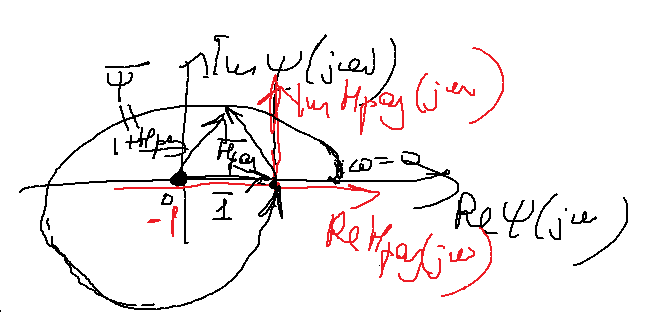
\includegraphics[width=.4\linewidth]{lec6/20_nyquist_godograph}

$ H_{\text{разомкн}} = \frac{\alpha}{\beta} $, порядок числителя, как правило, меньше порядка знаменателя $ \Rightarrow $ при $ \omega \to \infty $ $ H_{\text{разомкн}} \to 0 $.


Примеры.
Пусть $ l = 0 $ (тогда для устойчивости нужно ноль оборотов вокруг точки $ (-1;0) $).

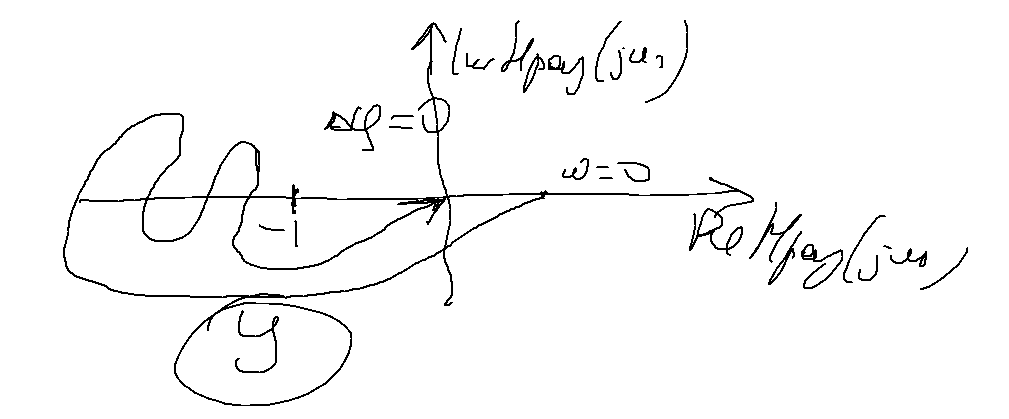
\includegraphics[width=.4\linewidth]{lec6/21_nyquist_godograph_stable1}
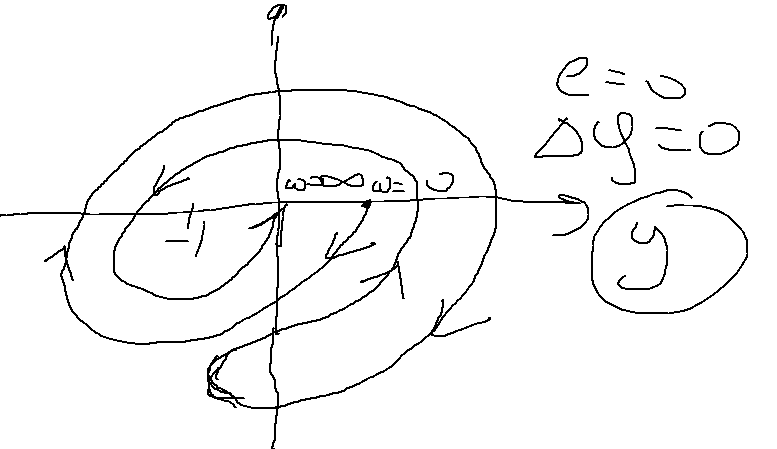
\includegraphics[width=.4\linewidth]{lec6/22_nyquist_godograph_stable2}

Число неустойчивых корней знаменателя $ l = 0 $, годограф делает ноль оборотов вокруг точки $ (-1;0) $ (на обеих картинках), и обе системы устойчивы.

\subsubsection{Геометрическое правило Цыпкина}

Это правило позволяет определить число оборотов вокруг точки $ (-1;0) $ по алгоритму.

Будем считать число пересечений с лучом $ ( - \infty; -1 ]) $ на вещественной оси: если пересекаем из второго квадранта в третий, добавляем +1; из третьего во второй -- -1; если стартуем из точки на отрицательной вещественной полуоси, добавляем + или $ - \frac{1}{2} $ в зависимости от того, в какую сторону стартуем.

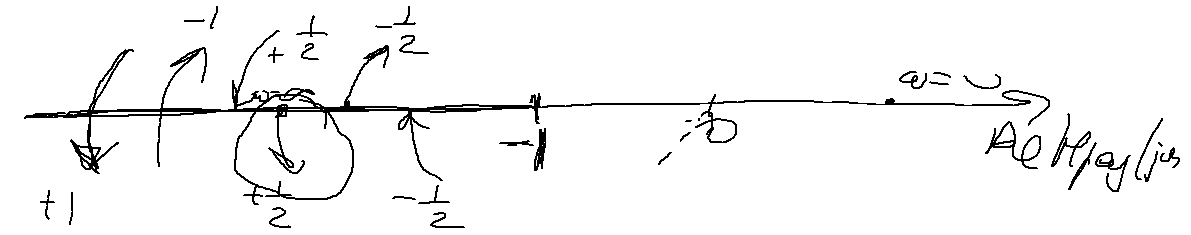
\includegraphics[width=\linewidth]{lec6/23_tsipkin}

Критерий Найквиста в интерпретации Цыпкина: система устойчива $ \Leftrightarrow  \sum X = \frac{l}{2}$ (число пересечений годографа с осью абсцисс левее $ -1 $ равняетая $ \frac{l}{2} $).

Пример.
$$ H_{\text{раз}}(p) = \frac{2}{p-1} \Rightarrow l = 1 $$
$$ H_{\text{раз}}(j \omega) = \frac{2}{j \omega - 1} = \frac{-2 - 2 j \omega}{\omega^2 + 1} $$
Годограф:

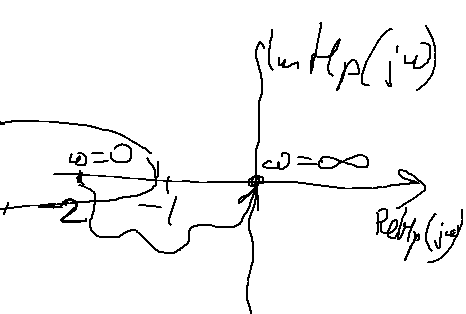
\includegraphics[width=.4\linewidth]{lec6/24_tsipkin_example1}

Сумма пересечений $ \sum X = \frac{1}{2}  $, $ l = 1 $ $ \Rightarrow $ система устойчива!

Проверка (по критерию Михайлова):
$$ \alpha_{\text{з}} = \alpha + \beta = (p - 1) + 2 = p + 1 $$
Это устойчивый многочлен!

\subsubsection{Критические случаи}
У критерия Михайлова нет особых случаев.
У критерия Найквиста есть.

\textbf{Первый критический случай:}

$ H_{\text{раз}} = \frac{\beta(p)}{p^s \alpha(p)} $ -- плохо, т. к.
$$ H_{\text{раз}}(j \omega)|_{\omega \to 0} \to \infty $$
Тогда принцип аргумента применить нельзя, $ \Delta \arg (1 + H_{\text{раз}}(j \omega)) |_0^{\infty} $ не  определена.

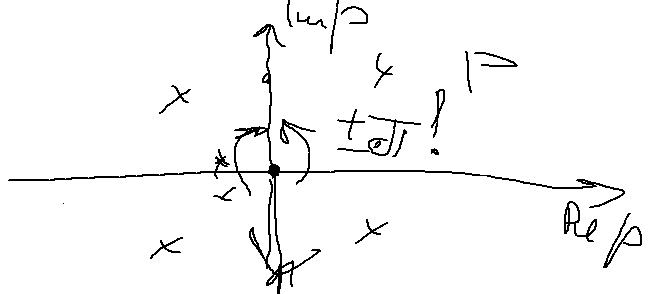
\includegraphics[width=.4\linewidth]{lec6/25_critical1}

Как быть?

Изменим траекторию: будем идти не везде по мнимой оси, а обойдём корень, который расположен на этой оси, по дуге очень маленькой окружности (маленькой, чтобы не захватить дугой другие корни).

Принцип аргумента при этом сохраняется, приращение аргумента от всех корней слева всё так же будет $ + \pi $, от правых $ - \pi $.
Раньше было так:
 $$ \Delta \arg \alpha(j \omega) |_{- \infty}^\infty = \pi (n - 2 l) $$
Обходим неприятную точку $ (0;0) $ справа (слева нам неудобно).
Теперь становится так (модификация принципа аргумента для знаменателя): $\Delta \arg \alpha(p) |_{\text{trajectory}}$

$$ trajectory = \begin{cases}
    j \omega, \omega < - \varepsilon or \omega > \varepsilon \\
    \varepsilon e^{- j \frac{\pi \omega}{ 2 \varepsilon}}, \omega \in [- \varepsilon; \varepsilon]
\end{cases} $$
Если $ \omega = \pm \varepsilon $, мы в точке $ (0; \pm \varepsilon) $; $ \omega = 0 \Rightarrow (\varepsilon, 0) $

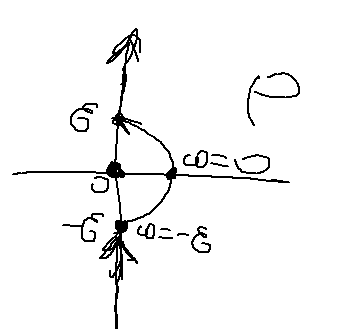
\includegraphics[width=.3\linewidth]{lec6/27_critical_omega_path}

\begin{align*}
    \Delta \arg [1 + H_{\text{раз}}(p)] |_{traject} & = \Delta \arg \alpha_{\text{з}}(p)|_{traject} - \Delta \arg \alpha (p) |_{traject} \\
    & = \pi(n-2m) - \pi(n-2l) \overset{m=0}= 2 \pi l
\end{align*}

Если же проходим половину траектории от $ \omega = 0 $ до $ \infty $:
$$ \Delta \arg [1 + H_{\text{раз}}(p)] |_{traject / 2} = \pi l = 2 \pi \cdot \frac{l}{2} $$

Как строить годограф?

$$ H_{\text{раз}}(p) = \begin{cases}
    H_{\text{раз}}(j \omega), \omega > \varepsilon \\
    H_{\text{раз}}(p), p = \varepsilon e^{j \frac{\pi}{2} \frac{\omega}{\varepsilon}}
\end{cases} $$

Что происходит вблизи нуля?
Пример:

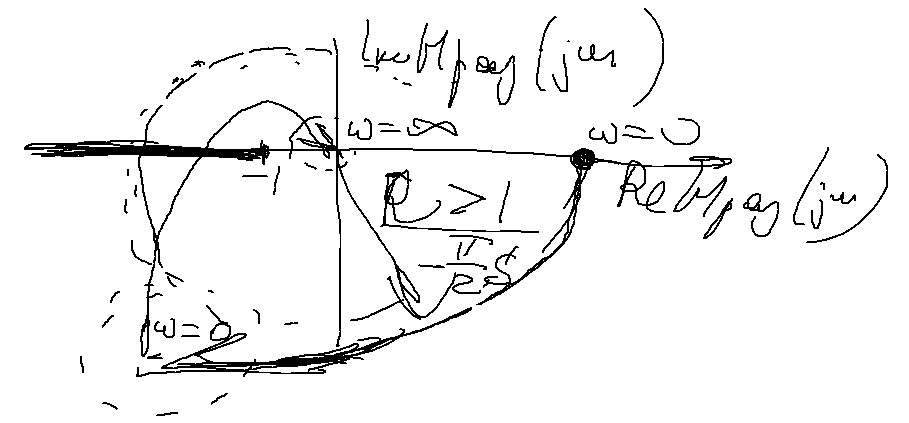
\includegraphics[width=.5\linewidth]{lec6/28_critical_integrator_godograph}

$$ H_{\text{раз}}(p) |_{traj / 2, \varepsilon \to 0} = \begin{cases}
    H_{\text{раз}}(j \omega), \omega > \varepsilon \\
    \frac{\beta(0)}{\varepsilon^s e^{j \frac{\pi}{2} s \frac{\omega}{\varepsilon}} \alpha(0)}, 0 \le \omega \le \varepsilon
\end{cases} $$

Вблизи нуля можно представить $ H_{\text{раз}} = \frac{\beta(p)}{p^s \alpha(p)}  $  в виде $ \frac{\beta(0)}{\alpha(0)} R e^{- j \phi} $, где $ R = \frac{1}{\varepsilon^s} \underset{\varepsilon \to 0}\to \infty $, $ \phi \in \left[ 0; \frac{\pi}{2}s \right] $

Т. о. надо дополнить годограф дугой бесконечно большого радиуса с фазой $ - \frac{\pi}{2}s $ ($ s $ -- кратность нуля как корня знаменателя), которая должна начинаться на положительной полуоси.
Найдя эту траекторию, считаем число пересечений.

Замечание: для применения правила Цыпкина достаточно брать не бесконечно большую дугу, а любую с радиусом $ R > 1 $, чтобы захватить точку $ (-1;0) $. \\

Пример: интегратор.
$$ H_{\text{раз}} = \frac{1}{p} $$
Годограф интегратора, напомним, таков:

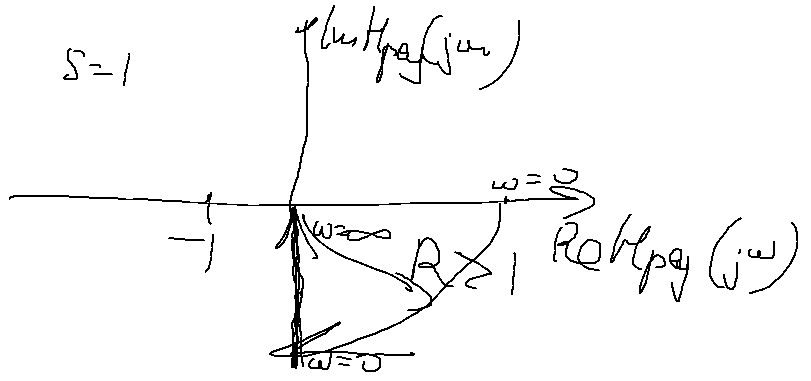
\includegraphics[width=.4\linewidth]{lec6/29_critical_example}

$ s = 1, l = 0 $.
Дополняем эту траекторию дугой так, чтобы движение по дуге осуществлялось по часовой стрелке.
Сумма пересечений левее $ (-1;0) $ равна нулю и $ l=0 \Rightarrow $ система устойчива.

Проверка:
$$ \alpha_{\text{з}} = p + 1 $$
Система устойчива! \\

Ещё один пример:
\begin{align*}
    & H_{\text{раз}} = \frac{1}{p^3} \\
    & H_{\text{раз}}(j \omega) = \frac{1}{(j \omega)^3} = \frac{j}{\omega^3}
\end{align*}

$ s = 3 \Rightarrow $ достраиваем годограф в районе точки $ \omega = 0 $ дугой с углом $ \Delta \phi = - \frac{3}{2}\pi $.

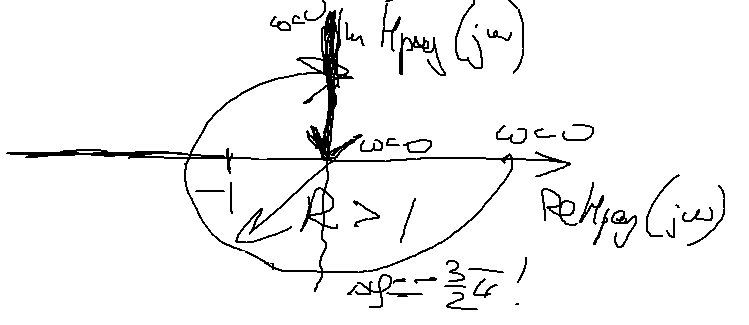
\includegraphics[width=.4\linewidth]{lec6/30_critical_example2}

Число пересечений $ \sum X = -1 \ne \frac{l}{2} = 0 $.

Проверка: $ \alpha_{\text{з}} = p^3 + 1 $; корни расположены на единичной окружности (см. рисунок ниже) и не все в левой полуплоскости $ \Rightarrow $ система неустойчива!

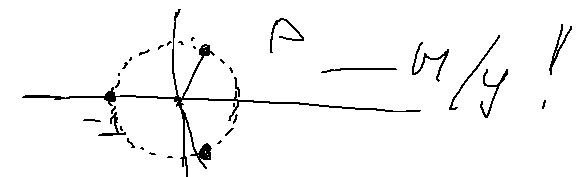
\includegraphics[width=.4\linewidth]{lec6/31_critical_example2_roots}

\textbf{Второй критический случай:} когда есть комплексно сопряжённые чисто мнимые корни знаменателя, т. е. передаточная функция
$$ H_{\text{раз}}(p) = \frac{\beta(p)}{\prod(p^2 + \omega_\mu^2) \alpha(p)} $$

Корни:

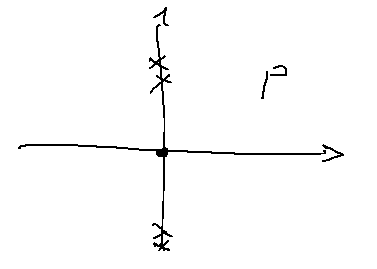
\includegraphics[width=.4\linewidth]{lec6/33_critical_example3_roots}

Скобка в точке $ \omega_\mu $ меняет знак $ \Rightarrow $ <<прыжок>> на $\pi$ или $-\pi$, разрыв.

Что делать?
Выход: обходим корень по дуге бесконечно малого радиуса.

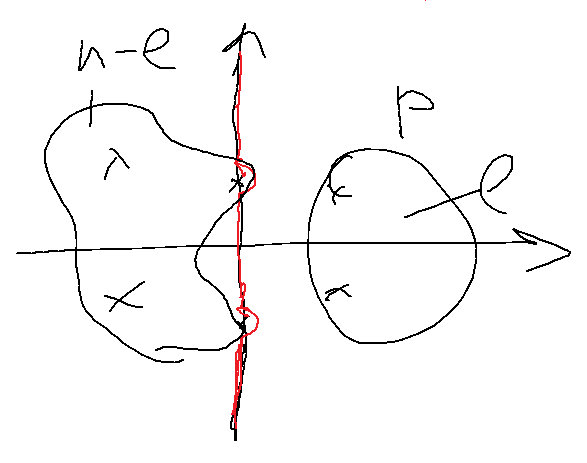
\includegraphics[width=.4\linewidth]{lec6/34_critical_example3_roots2}

Тогда изменение аргумента вспомогательной функции от $p$ всё так же $ 2 \pi l $:

$$ \Delta \arg \left[ 1 + H_{\text{раз}}(p) \right]|_{traj} = 2 \pi l $$
Из симметрии, как и раньше, можно взять половину траектории:
$$ \Delta \arg \left[ 1 + H_{\text{раз}}(p) \right]|_{traj / 2 } = \pi l = 2 \pi \frac{l}{2} $$
Для каждого разрыва дополняем годограф дугой с углом $ - \pi $.

Годограф выглядит теперь так:

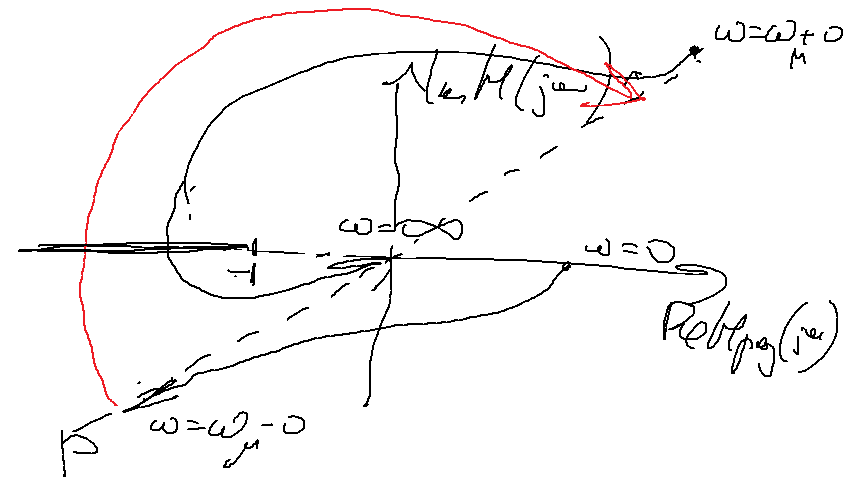
\includegraphics[width=.4\linewidth]{lec6/32_critical_example3_godograph}

Итак, если у нас второй критический случай (в знаменателе есть чисто мнимые корни), то дополняем годограф дугой бесконечно большого радиуса с радиусом $ - \pi \cdot \text{кратность корня} $, после чего уже можно пользоваться правилом Цыпкина. \\

Пример.
\begin{align*}
    & H_{\text{раз}}(p) = \frac{p}{p^2 + 1} \Rightarrow \thickspace l = 0  \\
    & p_{1,2} = \pm j \\
    & H_{\text{раз}}(j \omega) = \frac{j \omega}{1 - \omega^2}
\end{align*}

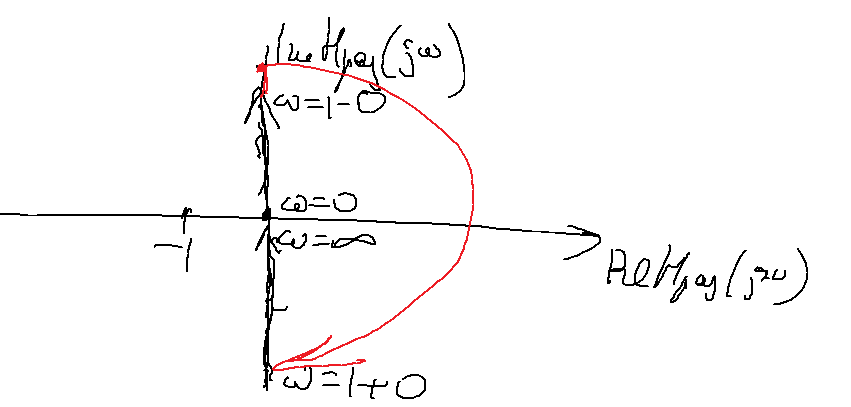
\includegraphics[width=.4\linewidth]{lec6/35_critical_example4}

Число пересечений левее $ -1 $: $ \sum X = 0 = \frac{l}{2} $ $ \Rightarrow $ система устойчива. \\

Проверка: $ \alpha_{\text{з}} = p^2 + p + 1 $ $ \Rightarrow $ система устойчива.

Второй пример -- то же самое, но со знаком минус:
\begin{align*}
    & H_{\text{раз}}(p) = \frac{-p}{p^2 + 1}, \thickspace l = 0  \\
    & \text{Сразу запишем: } \alpha_{\text{з}} = p^2 - p - 1 \Rightarrow \text{ неустойчива} \\
    & H_{\text{раз}}(j \omega) = \frac{- j \omega}{1 - \omega^2}
\end{align*}

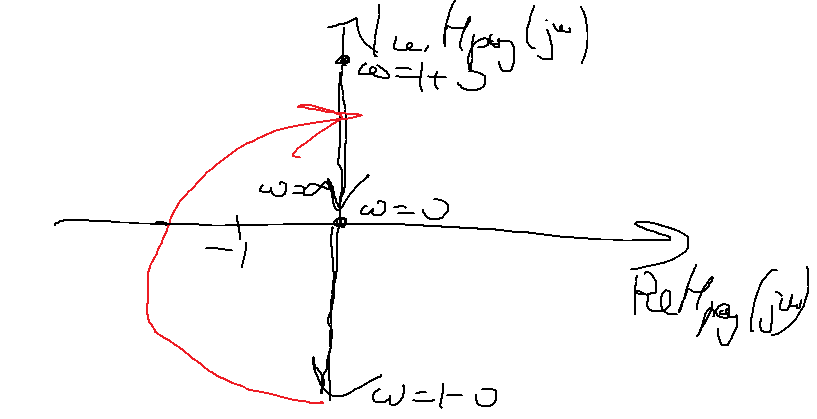
\includegraphics[width=.4\linewidth]{lec6/36_critical_example5}

Число пересечений $ \sum X = -1 \ne \frac{l}{2} \Rightarrow $ неустойчива!

\subsubsection{Границы устойчивости в критерии Найквиста}

Если в критерии Михайлова точка, подозрительная на границу устойчивости -- $ (0;0) $, то здесь -- $ (-1;0) $.
Как исследовать?
Точно так же: пошевелить.

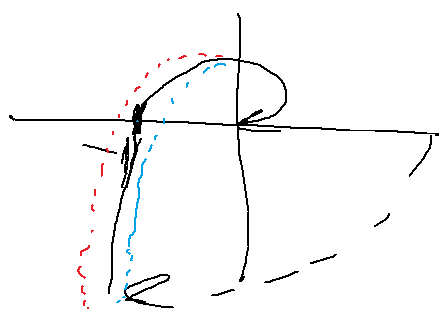
\includegraphics[width=.4\linewidth]{lec6/37_nyquist_boundary}

Пример:
\begin{align*}
    & H_{\text{раз}} = \frac{K}{p(T_1 p + 1)(T_2 p + 1)}; K_{\text{крит}} = ? \\
    & l = 0 \\
    & H_{\text{раз}}(j \omega) = \frac{K}{j \omega(1 + j \omega T_1)(1 + j \omega T_2)} \\
\end{align*}
Удобно представить в полярных координатах:
\begin{align*}
    & | H_{\text{раз}}(j \omega) | = \frac{K}{\omega \sqrt{(1 + \omega^2 T_1^2}\sqrt{1 + \omega^2 T_2^2}} \\
    & \phi = 0 - \left[\frac{\pi}{2} + \arctan \omega T_1 + \arctan \omega T_2 \right]
\end{align*}

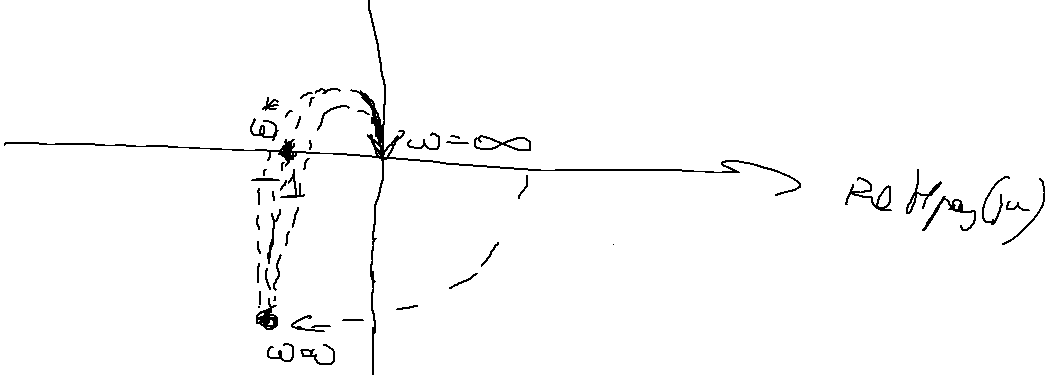
\includegraphics[width=.6\linewidth]{lec6/39_nyquist_bound_example}
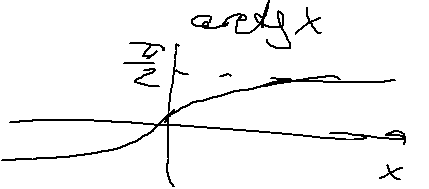
\includegraphics[width=.3\linewidth]{lec6/38_atan}

Когда $ K = K_{\text{крит}} $, годограф проходит через $ -1 $.

Пусть это пересечение происходит в точке $ \omega^* $.
Решаем уравнение:

\begin{align*}
    & \phi(\omega^*) = - \pi \\
    & \arctan \omega T_1 + \arctan \omega T_2 = \frac{\pi}{2} \\
    & \frac{\omega T_1 + \omega T_2}{1 - \omega^2 T_1 T_2} = \infty \\
    & \omega^{*2} = \frac{1}{T_1 T_2} \\
    & | H_{\text{раз}}(j \omega^*) | = 1 = \frac{K_{\text{крит}}}{\omega^* \sqrt{1 + \frac{T_1^2}{T_1 T_2}} \sqrt{1 + \frac{T_2^2}{T_1 T_2}}} = \frac{K_{\text{крит}}}{\frac{T_1 + T_2}{T_1 T_2}} \\
    & K_{\text{крит}} = \frac{T_1 + T_2}{T_1 T_2} \text{ (совпадает с результатом, полученным по критерию Михайлова)} \\
\end{align*}

\end{document}
